\documentclass{standalone}
\usepackage{tikz}
\usetikzlibrary{shapes.misc, positioning, arrows.meta, calc}

\begin{document}

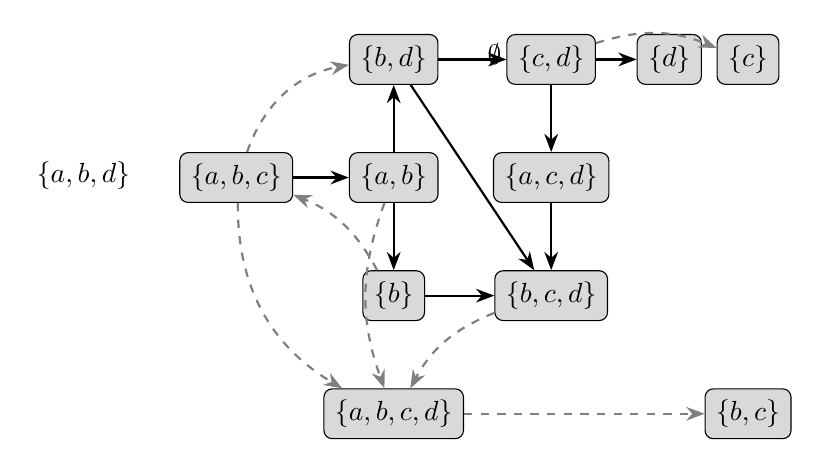
\begin{tikzpicture}[
  node distance=1.5cm,
  set/.style={draw, fill=gray!30, rounded corners=3pt, inner sep=4pt},
  transition/.style={->, >=Stealth, thick},
  dashed transition/.style={transition, dashed, gray}
]

% Define nodes (sets)
\node[set] (ab) at (0,0) {$\{a,b\}$};
\node[set] (abc) at (-2,0) {$\{a,b,c\}$};
\node[set] (abd) at (0,1.5) {$\{b,d\}$};
\node[set] (b) at (0,-1.5) {$\{b\}$};
\node[set] (bcd) at (2,-1.5) {$\{b,c,d\}$};
\node[set] (cd) at (2,1.5) {$\{c,d\}$};
\node[set] (acd) at (2,0) {$\{a,c,d\}$};
\node[set] (abcd) at (0,-3) {$\{a,b,c,d\}$};
\node[set] (d) at (3.5,1.5) {$\{d\}$};
\node[set] (c) at (4.5,1.5) {$\{c\}$};
\node[set] (bc) at (4.5,-3) {$\{b,c\}$};

% Add text above nodes for some sets
\node[left=0.5cm of abc.north west, anchor=north east] {$\{a,b,d\}$};
\node[right=0.5cm of abd.north east, anchor=north west] {$\emptyset$};

% Draw solid transitions
\draw[transition] (abc) -- (ab);
\draw[transition] (ab) -- (abd);
\draw[transition] (ab) -- (b);
\draw[transition] (abd) -- (cd);
\draw[transition] (abd) -- (bcd);
\draw[transition] (b) -- (bcd);
\draw[transition] (cd) -- (d);
\draw[transition] (cd) -- (acd);
\draw[transition] (acd) -- (bcd);

% Draw dashed transitions
\draw[dashed transition] (abc) to[bend left=30] (abd);
\draw[dashed transition] (abc) to[bend right=30] (abcd);
\draw[dashed transition] (ab) to[bend right=20] (abcd);
\draw[dashed transition] (b) to[bend right=20] (abc);
\draw[dashed transition] (cd) to[bend left=20] (c);
\draw[dashed transition] (abcd) -- (bc);
\draw[dashed transition] (bcd) to[bend right=20] (abcd);

\end{tikzpicture}

\end{document}